\documentclass[conference,compsoc]{IEEEtran}

% *** CITATION PACKAGES ***
%
\ifCLASSOPTIONcompsoc
  % IEEE Computer Society needs nocompress option
  % requires cite.sty v4.0 or later (November 2003)
  \usepackage[nocompress]{cite}
\else
  % normal IEEE
  \usepackage{cite}
\fi
% cite.sty was written by Donald Arseneau
% V1.6 and later of IEEEtran pre-defines the format of the cite.sty package
% \cite{} output to follow that of the IEEE. Loading the cite package will
% result in citation numbers being automatically sorted and properly
% "compressed/ranged". e.g., [1], [9], [2], [7], [5], [6] without using
% cite.sty will become [1], [2], [5]--[7], [9] using cite.sty. cite.sty's
% \cite will automatically add leading space, if needed. Use cite.sty's
% noadjust option (cite.sty V3.8 and later) if you want to turn this off
% such as if a citation ever needs to be enclosed in parenthesis.
% cite.sty is already installed on most LaTeX systems. Be sure and use
% version 5.0 (2009-03-20) and later if using hyperref.sty.
% The latest version can be obtained at:
% http://www.ctan.org/pkg/cite
% The documentation is contained in the cite.sty file itself.
%
% Note that some packages require special options to format as the Computer
% Society requires. In particular, Computer Society  papers do not use
% compressed citation ranges as is done in typical IEEE papers
% (e.g., [1]-[4]). Instead, they list every citation separately in order
% (e.g., [1], [2], [3], [4]). To get the latter we need to load the cite
% package with the nocompress option which is supported by cite.sty v4.0
% and later.





% *** GRAPHICS RELATED PACKAGES ***
%
\ifCLASSINFOpdf
  % \usepackage[pdftex]{graphicx}
  % declare the path(s) where your graphic files are
  % \graphicspath{{../pdf/}{../jpeg/}}
  % and their extensions so you won't have to specify these with
  % every instance of \includegraphics
  % \DeclareGraphicsExtensions{.pdf,.jpeg,.png}
\else
  % or other class option (dvipsone, dvipdf, if not using dvips). graphicx
  % will default to the driver specified in the system graphics.cfg if no
  % driver is specified.
  % \usepackage[dvips]{graphicx}
  % declare the path(s) where your graphic files are
  % \graphicspath{{../eps/}}
  % and their extensions so you won't have to specify these with
  % every instance of \includegraphics
  % \DeclareGraphicsExtensions{.eps}
\fi
% graphicx was written by David Carlisle and Sebastian Rahtz. It is
% required if you want graphics, photos, etc. graphicx.sty is already
% installed on most LaTeX systems. The latest version and documentation
% can be obtained at: 
% http://www.ctan.org/pkg/graphicx
% Another good source of documentation is "Using Imported Graphics in
% LaTeX2e" by Keith Reckdahl which can be found at:
% http://www.ctan.org/pkg/epslatex
%
% latex, and pdflatex in dvi mode, support graphics in encapsulated
% postscript (.eps) format. pdflatex in pdf mode supports graphics
% in .pdf, .jpeg, .png and .mps (metapost) formats. Users should ensure
% that all non-photo figures use a vector format (.eps, .pdf, .mps) and
% not a bitmapped formats (.jpeg, .png). The IEEE frowns on bitmapped formats
% which can result in "jaggedy"/blurry rendering of lines and letters as
% well as large increases in file sizes.
%
% You can find documentation about the pdfTeX application at:
% http://www.tug.org/applications/pdftex





% *** MATH PACKAGES ***
%
\usepackage{graphicx} 
\usepackage{amsmath}
% A popular package from the American Mathematical Society that provides
% many useful and powerful commands for dealing with mathematics.
%
% Note that the amsmath package sets \interdisplaylinepenalty to 10000
% thus preventing page breaks from occurring within multiline equations. Use:
%\interdisplaylinepenalty=2500
% after loading amsmath to restore such page breaks as IEEEtran.cls normally
% does. amsmath.sty is already installed on most LaTeX systems. The latest
% version and documentation can be obtained at:
% http://www.ctan.org/pkg/amsmath





% *** SPECIALIZED LIST PACKAGES ***
%
\usepackage{algorithm}
\usepackage{algorithmic}
\renewcommand{\algorithmicrequire}{\textbf{Input:}}
\renewcommand{\algorithmicensure}{\textbf{Output:}}

% algorithmic.sty was written by Peter Williams and Rogerio Brito.
% This package provides an algorithmic environment fo describing algorithms.
% You can use the algorithmic environment in-text or within a figure
% environment to provide for a floating algorithm. Do NOT use the algorithm
% floating environment provided by algorithm.sty (by the same authors) or
% algorithm2e.sty (by Christophe Fiorio) as the IEEE does not use dedicated
% algorithm float types and packages that provide these will not provide
% correct IEEE style captions. The latest version and documentation of
% algorithmic.sty can be obtained at:
% http://www.ctan.org/pkg/algorithms
% Also of interest may be the (relatively newer and more customizable)
% algorithmicx.sty package by Szasz Janos:
% http://www.ctan.org/pkg/algorithmicx






% *** ALIGNMENT PACKAGES ***
%
\usepackage{array}
% Frank Mittelbach's and David Carlisle's array.sty patches and improves
% the standard LaTeX2e array and tabular environments to provide better
% appearance and additional user controls. As the default LaTeX2e table
% generation code is lacking to the point of almost being broken with
% respect to the quality of the end results, all users are strongly
% advised to use an enhanced (at the very least that provided by array.sty)
% set of table tools. array.sty is already installed on most systems. The
% latest version and documentation can be obtained at:
% http://www.ctan.org/pkg/array


% IEEEtran contains the IEEEeqnarray family of commands that can be used to
% generate multiline equations as well as matrices, tables, etc., of high
% quality.




% *** SUBFIGURE PACKAGES ***
%\ifCLASSOPTIONcompsoc
%  \usepackage[caption=false,font=footnotesize,labelfont=sf,textfont=sf]{subfig}
%\else
%  \usepackage[caption=false,font=footnotesize]{subfig}
%\fi
% subfig.sty, written by Steven Douglas Cochran, is the modern replacement
% for subfigure.sty, the latter of which is no longer maintained and is
% incompatible with some LaTeX packages including fixltx2e. However,
% subfig.sty requires and automatically loads Axel Sommerfeldt's caption.sty
% which will override IEEEtran.cls' handling of captions and this will result
% in non-IEEE style figure/table captions. To prevent this problem, be sure
% and invoke subfig.sty's "caption=false" package option (available since
% subfig.sty version 1.3, 2005/06/28) as this is will preserve IEEEtran.cls
% handling of captions.
% Note that the Computer Society format requires a sans serif font rather
% than the serif font used in traditional IEEE formatting and thus the need
% to invoke different subfig.sty package options depending on whether
% compsoc mode has been enabled.
%
% The latest version and documentation of subfig.sty can be obtained at:
% http://www.ctan.org/pkg/subfig




% *** FLOAT PACKAGES ***
%
%\usepackage{fixltx2e}
% fixltx2e, the successor to the earlier fix2col.sty, was written by
% Frank Mittelbach and David Carlisle. This package corrects a few problems
% in the LaTeX2e kernel, the most notable of which is that in current
% LaTeX2e releases, the ordering of single and double column floats is not
% guaranteed to be preserved. Thus, an unpatched LaTeX2e can allow a
% single column figure to be placed prior to an earlier double column
% figure.
% Be aware that LaTeX2e kernels dated 2015 and later have fixltx2e.sty's
% corrections already built into the system in which case a warning will
% be issued if an attempt is made to load fixltx2e.sty as it is no longer
% needed.
% The latest version and documentation can be found at:
% http://www.ctan.org/pkg/fixltx2e


%\usepackage{stfloats}
% stfloats.sty was written by Sigitas Tolusis. This package gives LaTeX2e
% the ability to do double column floats at the bottom of the page as well
% as the top. (e.g., "\begin{figure*}[!b]" is not normally possible in
% LaTeX2e). It also provides a command:
%\fnbelowfloat
% to enable the placement of footnotes below bottom floats (the standard
% LaTeX2e kernel puts them above bottom floats). This is an invasive package
% which rewrites many portions of the LaTeX2e float routines. It may not work
% with other packages that modify the LaTeX2e float routines. The latest
% version and documentation can be obtained at:
% http://www.ctan.org/pkg/stfloats
% Do not use the stfloats baselinefloat ability as the IEEE does not allow
% \baselineskip to stretch. Authors submitting work to the IEEE should note
% that the IEEE rarely uses double column equations and that authors should try
% to avoid such use. Do not be tempted to use the cuted.sty or midfloat.sty
% packages (also by Sigitas Tolusis) as the IEEE does not format its papers in
% such ways.
% Do not attempt to use stfloats with fixltx2e as they are incompatible.
% Instead, use Morten Hogholm'a dblfloatfix which combines the features
% of both fixltx2e and stfloats:
%
% \usepackage{dblfloatfix}
% The latest version can be found at:
% http://www.ctan.org/pkg/dblfloatfix




% *** PDF, URL AND HYPERLINK PACKAGES ***
%
\usepackage{url}
% url.sty was written by Donald Arseneau. It provides better support for
% handling and breaking URLs. url.sty is already installed on most LaTeX
% systems. The latest version and documentation can be obtained at:
% http://www.ctan.org/pkg/url
% Basically, \url{my_url_here}.




% *** Do not adjust lengths that control margins, column widths, etc. ***
% *** Do not use packages that alter fonts (such as pslatex).         ***
% There should be no need to do such things with IEEEtran.cls V1.6 and later.
% (Unless specifically asked to do so by the journal or conference you plan
% to submit to, of course. )



% correct bad hyphenation here
\hyphenation{op-tical net-works semi-conduc-tor}


\begin{document}
%
% paper title
% Titles are generally capitalized except for words such as a, an, and, as,
% at, but, by, for, in, nor, of, on, or, the, to and up, which are usually
% not capitalized unless they are the first or last word of the title.
% Linebreaks \\ can be used within to get better formatting as desired.
% Do not put math or special symbols in the title.
\title{Machine learning based queuing time prediction of batch scheduler on supercomputers}


% author names and affiliations
% use a multiple column layout for up to three different
% affiliations
\author{\IEEEauthorblockN{Bowen Zhang, \	Xingyu Chen, \	Zengyi Wang}
\\
\IEEEauthorblockA{Southern University of Science and Technology\\
Department of Computer Science and Engineering
}}


% conference papers do not typically use \thanks and this command
% is locked out in conference mode. If really needed, such as for
% the acknowledgment of grants, issue a \IEEEoverridecommandlockouts
% after \documentclass

% for over three affiliations, or if they all won't fit within the width
% of the page (and note that there is less available width in this regard for
% compsoc conferences compared to traditional conferences), use this
% alternative format:
% 
%\author{\IEEEauthorblockN{Michael Shell\IEEEauthorrefmark{1},
%Homer Simpson\IEEEauthorrefmark{2},
%James Kirk\IEEEauthorrefmark{3}, 
%Montgomery Scott\IEEEauthorrefmark{3} and
%Eldon Tyrell\IEEEauthorrefmark{4}}
%\IEEEauthorblockA{\IEEEauthorrefmark{1}School of Electrical and Computer Engineering\\
%Georgia Institute of Technology,
%Atlanta, Georgia 30332--0250\\ Email: see http://www.michaelshell.org/contact.html}
%\IEEEauthorblockA{\IEEEauthorrefmark{2}Twentieth Century Fox, Springfield, USA\\
%Email: homer@thesimpsons.com}
%\IEEEauthorblockA{\IEEEauthorrefmark{3}Starfleet Academy, San Francisco, California 96678-2391\\
%Telephone: (800) 555--1212, Fax: (888) 555--1212}
%\IEEEauthorblockA{\IEEEauthorrefmark{4}Tyrell Inc., 123 Replicant Street, Los Angeles, California 90210--4321}}




% use for special paper notices
%\IEEEspecialpapernotice{(Invited Paper)}




% make the title area
\maketitle

% As a general rule, do not put math, special symbols or citations
% in the abstract
%\begin{abstract}

%\end{abstract}

% no keywords




% For peer review papers, you can put extra information on the cover
% page as needed:
% \ifCLASSOPTIONpeerreview
% \begin{center} \bfseries EDICS Category: 3-BBND \end{center}
% \fi
%
% For peerreview papers, this IEEEtran command inserts a page break and
% creates the second title. It will be ignored for other modes.
\IEEEpeerreviewmaketitle

% An example of a floating figure using the graphicx package.
% Note that \label must occur AFTER (or within) \caption.
% For figures, \caption should occur after the \includegraphics.
% Note that IEEEtran v1.7 and later has special internal code that
% is designed to preserve the operation of \label within \caption
% even when the captionsoff option is in effect. However, because
% of issues like this, it may be the safest practice to put all your
% \label just after \caption rather than within \caption{}.
%
% Reminder: the "draftcls" or "draftclsnofoot", not "draft", class
% option should be used if it is desired that the figures are to be
% displayed while in draft mode.
%
%\begin{figure}[!t]
%\centering
%\includegraphics[width=2.5in]{myfigure}
% where an .eps filename suffix will be assumed under latex, 
% and a .pdf suffix will be assumed for pdflatex; or what has been declared
% via \DeclareGraphicsExtensions.
%\caption{Simulation results for the network.}
%\label{fig_sim}
%\end{figure}

% Note that the IEEE typically puts floats only at the top, even when this
% results in a large percentage of a column being occupied by floats.


% An example of a double column floating figure using two subfigures.
% (The subfig.sty package must be loaded for this to work.)
% The subfigure \label commands are set within each subfloat command,
% and the \label for the overall figure must come after \caption.
% \hfil is used as a separator to get equal spacing.
% Watch out that the combined width of all the subfigures on a 
% line do not exceed the text width or a line break will occur.
%
%\begin{figure*}[!t]
%\centering
%\subfloat[Case I]{\includegraphics[width=2.5in]{box}%
%\label{fig_first_case}}
%\hfil
%\subfloat[Case II]{\includegraphics[width=2.5in]{box}%
%\label{fig_second_case}}
%\caption{Simulation results for the network.}
%\label{fig_sim}
%\end{figure*}
%
% Note that often IEEE papers with subfigures do not employ subfigure
% captions (using the optional argument to \subfloat[]), but instead will
% reference/describe all of them (a), (b), etc., within the main caption.
% Be aware that for subfig.sty to generate the (a), (b), etc., subfigure
% labels, the optional argument to \subfloat must be present. If a
% subcaption is not desired, just leave its contents blank,
% e.g., \subfloat[].


% An example of a floating table. Note that, for IEEE style tables, the
% \caption command should come BEFORE the table and, given that table
% captions serve much like titles, are usually capitalized except for words
% such as a, an, and, as, at, but, by, for, in, nor, of, on, or, the, to
% and up, which are usually not capitalized unless they are the first or
% last word of the caption. Table text will default to \footnotesize as
% the IEEE normally uses this smaller font for tables.
% The \label must come after \caption as always.
%
%\begin{table}[!t]
%% increase table row spacing, adjust to taste
%\renewcommand{\arraystretch}{1.3}
% if using array.sty, it might be a good idea to tweak the value of
% \extrarowheight as needed to properly center the text within the cells
%\caption{An Example of a Table}
%\label{table_example}
%\centering
%% Some packages, such as MDW tools, offer better commands for making tables
%% than the plain LaTeX2e tabular which is used here.
%\begin{tabular}{|c||c|}
%\hline
%One & Two\\
%\hline
%Three & Four\\
%\hline
%\end{tabular}
%\end{table}


% Note that the IEEE does not put floats in the very first column
% - or typically anywhere on the first page for that matter. Also,
% in-text middle ("here") positioning is typically not used, but it
% is allowed and encouraged for Computer Society conferences (but
% not Computer Society journals). Most IEEE journals/conferences use
% top floats exclusively. 
% Note that, LaTeX2e, unlike IEEE journals/conferences, places
% footnotes above bottom floats. This can be corrected via the
% \fnbelowfloat command of the stfloats package.


\begin{abstract}
	
	To share high performance computing resources, HPC clusters queue jobs to provide computing services. Due to the limited computing resources, naturally there is the problem of queuing. The prediction of queuing time can improve the resource utilization of a HPC cluster. There are some elastic jobs which can be run on any number of nodes in parallel and there are frameworks (e.g., parsl) that enable jobs to be executed in parallel on multiple nodes. Knowing the exact queue time is important for these jobs in order to minimize the response time. Response time is queue time plus running time. Our study will explore machine learning models that can accurately predict queue time, and propose an architecture that can improve model accuracy by using similarity calculation. We'll also talk about what we're doing now.
	
\end{abstract}


\section{Introduction}
\subsection{Supercomputers}

Nowadays, with the increasing demand for computational resources in the field of basic science, people tend to use computers with extreme computational power to process programs, and such computers with extreme computational power are called supercomputers. Supercomputers contain thousands of computing resources (CPUs and GPUs), and users request the appropriate number of computing resources to process tasks for them according to their needs. Upon receiving resource requests from different users, the supercomputer runs a program called a scheduler to allocate the computing resources. In other words, the supercomputing center provides a shared pool of resources, each task occupies part of the resources when it is executed, and multiple tasks are scheduled by the scheduler to allocate computing resources according to certain rules in a queue.

\subsection{A scheduling technique to improve resource utilization}

There is a scheduling technique called backfill, which improves the resource utilization of the system. We define tasks that consume more computational resources as large tasks and tasks that consume fewer computational resources as small tasks. Backfill works by reserving resources for the execution of large tasks. At the same time, the time gaps generated during the execution of large tasks are used to prioritize the small tasks in the waiting queue so that they are executed before the large tasks. Reserving resources for tasks with more computational resources avoids long waiting time for large jobs, and prioritizing small jobs in the queue improves the response time of small tasks, both of which increase the number of working nodes and improve the resource utilization of the system.

\subsection{Motivation}

Overall, predicting the queuing time submitted to a supercomputer processing system is both important for users to schedule their jobs and can help the scheduler make informed scheduling decisions.

Users would gain many benefits if they could predict the queuing time for jobs on a batch processing system. First, the predicted time can help the user plan to manage its work and help the user try to avoid not being able to complete the work by the deadline. When the queue prediction time is known to be too long, the user can choose another queue, and this practice can also reduce the load on certain queues of the computer and make the load more balanced.

In addition, there is a class of jobs that can be executed in parallel on an arbitrary number of nodes, and there are frameworks (e.g., parsl \cite{babuji2019parsl}) that enable job to be executed in parallel on multiple nodes. For this class of jobs, it is important to know the waiting time for different number of node requests, which will determine how many nodes can be used to execute the job in parallel to achieve the shortest response time. Also, the scheduler can effectively use this prediction to make scheduling decisions and select the appropriate number of computational resources and queues for each computational job to improve the utilization of computational resources.

\subsection{Research Objectives}

Some previous papers have shown that it is possible to predict a bound of the queuing time of batch scheduled jobs. Today, machine learning makes it possible to analyze and predict large amounts of data more quickly and accurately. With the recent advance of machine learning methods, we will revisit this problem and see if we could use machine learning to predict the queuing time of batch schedulers more accurately. We will explore different machine learning methods in this project to perform different levels of predictions.

\subsection{Research Challenges}

First, it is impractical to obtain or infer the priority and scheduling algorithms of the jobs because most of the scheduling algorithms are not open source. It is difficult for us to know the exact workflow of most scheduling algorithms, adding difficulties to predicting queueing times.

In addition, predicting the queue wait time faces the difficulty that the wait time of a particular task depends partly on the future task arrivals and the execution of tasks at each compute node, which are unknowable at the time of prediction.

Also, the system has a backfill mechanism that causes a portion of small tasks to be executed earlier. This makes it more difficult to predict the waiting time of the queue.

\section{Related work}
The existing papers provide different prediction methods from different machine learning models. These methods can be broadly classified into two categories: the first category will calculate the similarity between tasks and group the tasks with similarity into one category. The execution time of that task is then predicted based on the execution time of similar tasks. The second category is to directly use a machine learning model to predict the execution time of a task.

The first class of methods is the most common in current research.W. Smith used this class of methods in \cite{smith1999resource} where summary statistics about the state of resources (e.g., number of running jobs and idle cpu) are used as attributes. In other work by W. Smith \cite{smitharticle}\cite{10.1007/3-540-47954-6_11}, runtime predictions are derived using historically similar runs, and these estimates are further used to simulate scheduling algorithms such as FCFS, LWF. Hui Li's\cite{li2005efficient} approach is to first classify tasks by similarity and then search them using a genetic algorithm to keep the relative prediction error between 0.35 - 0.70.

Unlike computing similarity, there are also studies that directly pass the data into a machine learning model directly to predict the queuing time. In a recent paper by Ju-Won Park\cite{park2022queue}, it used the HMM approach to improve the prediction accuracy of traditional algorithms by 60 percents. In Rajath Kumar's\cite{kumar2014prediction} work, he first predicts the waiting time of jobs using a dynamic k-nearest neighbor (kNN) approach. Then multiclass classification of all classes of jobs is performed using support vector machines. The probabilities obtained using the above two methods were used to provide a set of predicted waiting time ranges with probabilities. The scheduling policy designed based on this predicted time range reduced the average queuing wait time of jobs by 47 percents.

From the point of practical application, the result of the present work is still not very well. The error of categorical prediction or direct prediction is very large. For practical application, too large error is not acceptable. Our research is aimed at further improving the accuracy of predictions and making practical applications possible.

\section{Data Analysis}
In this section, we mainly focus on analyzing existing dataset and try to extract key information. Now we have completed the pre-processing and data analysis of theta cluster data.

There are many factors that effect queue time. It can be roughly divided into queue state, system state and job state. I will analyze theta data from these three directions. For the generalization of the model, we only analyze the default queue.
First, we defined the label and counted the number of different labels in Figure \ref{Fig:1}.

\begin{center}
	\begin{tabular}{||c|c|c|c||} 
		\hline
		Label & Meaning  \\ [0.5ex] 
		\hline\hline
		1 & less than one hour  \\ 
		\hline
		2 & 1 hour to 3 hours   \\
		\hline
		3 & 3 hours to 6 hours   \\
		\hline
		4 & 6 hours to 12 hours \\
		\hline
		5 & 12 hours to 24 hours   \\
		\hline
		6 & greater than one day  \\ 
		\hline
	\end{tabular}
	\label{table:1}
\end{center}

\begin{figure}[htbp]   %注意,这里设置是关键
	
	\centering
	
	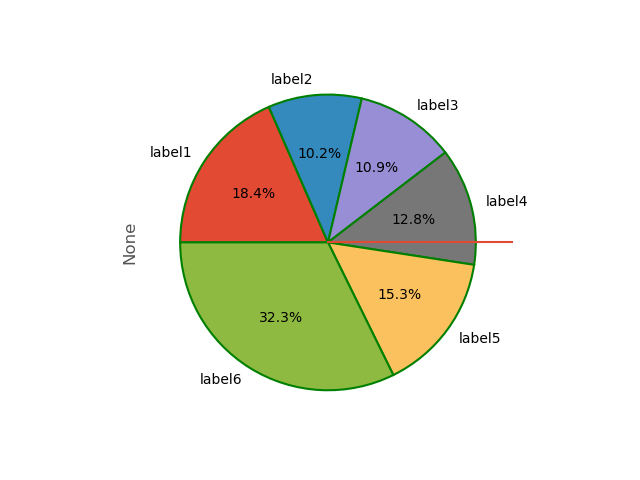
\includegraphics[width=\linewidth,scale=1.00]{myplot.png}
	
	%[]里面的参数自己可根据需要调整
	
	\caption{The distribution of label}
	
	\label{Fig:1}
	
\end{figure}
We find this distribution of Theta data odd, since jobs whose queue time are less than one hour usually account for more than 50\% of the total number of jobs in a cluster\cite{kumar2012identifying}, perhaps because theta smaller tasks typically use backfill queue.

\subsection{Job State}
Obviously, queue time has a certain relationship with request node. We do data analysis according to the request of each node number. Another factor that is obviously related to queue time is request run time. We will analyze the relationship between request node in Figure \ref{Fig:3}. and queue time and between request time in Figure \ref{Fig:2}. and queue time.
\begin{figure}[htbp]
	\begin{minipage}[t]{0.45\linewidth}
		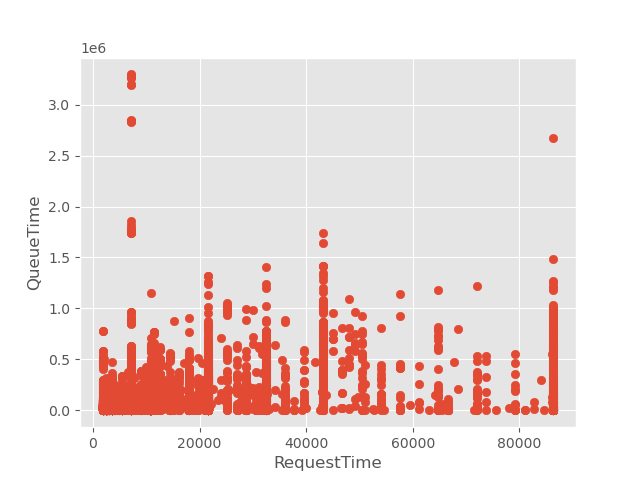
\includegraphics[width=\linewidth]{requesttimequeue.png} 
		\caption{scatter diagram request time with queue time} 
		\label{Fig:2}
	\end{minipage}%
	\hfill%
	\begin{minipage}[t]{0.45\linewidth}
		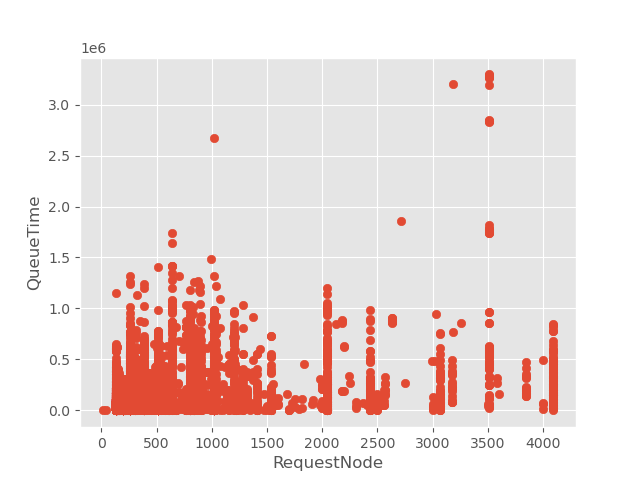
\includegraphics[width=\linewidth]{nodequeue.png}
		\caption{scatter diagram request node with queue time}
		\label{Fig:3}
	\end{minipage} 
\end{figure}

From the analysis, when request time is less than 40000s, queue time increases with request time. However, when the request time is greater than 40000s, Figure \ref{Fig:2} distribution is very disorganized and inconsistent with our expectations. In the scatter diagram of request Figure \ref{Fig:3} node and queue time, when the nodes are large, the distribution of queue time is also very scattered, generally low, with many outliers. The distribution of queue time when the request node is large does not conform to our expectations. When the request node is small, the distribution is more concentrated with fewer outliers, which is more consistent with our expectations.
The more resources applied by jobs, the more inconsistent with our intuitive prediction, and the more outliers, which may be due to the submitter notifying the supercomputer cluster manager in advance, or the account has priority. All these factors make it difficult for us to predict queue time using machine learning.

According to the above data analysis, we put forward a point of view: Jobs with larger resource scale are more influenced by human factors. To verify the above conjecture, we analyze the distribution of request time and request node Figure \ref{Fig:7}, and use request time * request node to measure the application of system resources for a jobs.
Then we make a scatter diagram request time * request node with queue time
\begin{figure}[htbp]
	\begin{minipage}[t]{0.45\linewidth}
		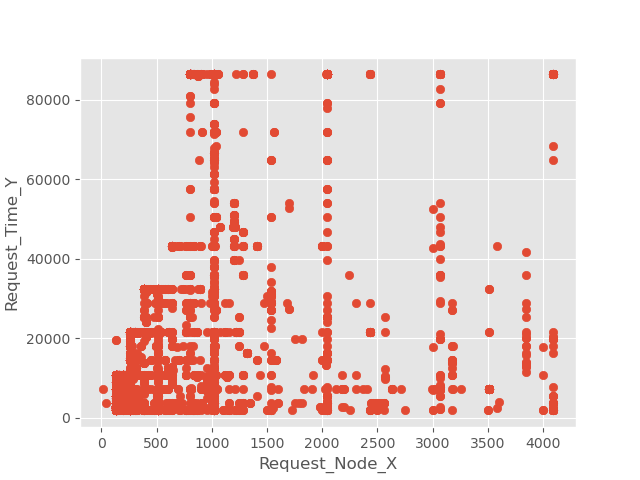
\includegraphics[width=\linewidth]{nodetime.png} 
		\caption{scatter diagram request time with request node} 
		\label{Fig:7}
	\end{minipage}%
	\hfill%
	\begin{minipage}[t]{0.45\linewidth}
		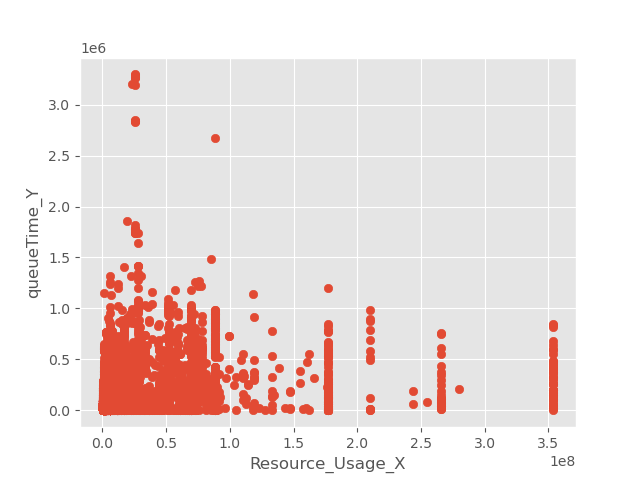
\includegraphics[width=\linewidth]{Resource.png}
		\caption{scatter diagram Resource with queue time}
		\label{Fig:8}
	\end{minipage} 
\end{figure}

According to data analysis Figure \ref{Fig:7}, when request node is less than 1000, the distribution of request time increases significantly in the area with large value with the increase of request node. When the request node is near 1000, the request time is evenly distributed. Subsequently, as the request node grows, the request time is more concentrated and distributed in the low/middle area. As can be seen from Figure \ref{Fig:8}, when the resource application of a Job is significantly larger than that of other Jobs, its waiting time will decrease significantly. This also proves the above conjecture.

\subsection{System/Queue State}
We use default queue as our dataset. Hardware resources corresponding to the default queue are not isolated. Therefore, the system state affects the queue time of the job to some extent. And there is no doubt that the state of the queue when a job is submitted affects the queue time of the job. Since we have not reached an agreement on the features of system state and queue state at present, I only use some features \ref{table:2} that I think are very typical here.

We defines two features for system state and queue state.
\begin{center}
	\resizebox{.95\columnwidth}{!}{
		\begin{tabular}{|cp{8cm}|c|} 
			\hline
			name & Meaning   \\ [0.5ex] 
			\hline\hline
			prpjobRankReqsize & The position of the target job in the list of running jobs in the system at
			the time of its entry sorted in increasing order of request sizes   \\ 
			\hline
			queueJobRankByReqsize & The position of the target job in the list of queue jobs in the default queue at
			the time of its entry sorted in increasing order of request sizes  \\
			\hline
		\end{tabular}
		\label{table:2}
	}
\end{center}
The reason why I use rank instead of the number of node applications is that for queue job list, the smaller the application node, the more likely the job will be backfilled first. The size is relative, so I use rank. For running job list, The size of a running job is also relative. A smaller job is more likely to be executed. After a running job ends, a certain number of nodes will be released, and we compare the number of released nodes with the number of job applications. The job will be executed only when the number of nodes released exceeds the number of applications. Figure \ref{Fig:4}. shows relationships between prpjobRankReqsize and queue time and Figure \ref{Fig:5}. shows relationships between queueJobRankByReqsize and queue time.


\begin{figure}[htbp]
	\begin{minipage}[t]{0.45\linewidth}
		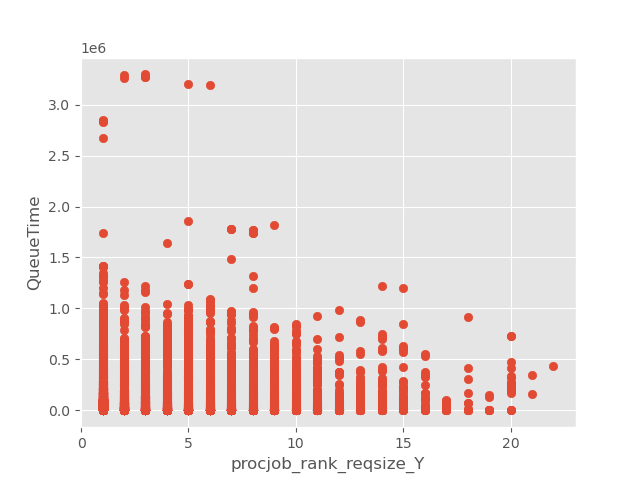
\includegraphics[width=\linewidth]{runningjobrank.png} 
		\caption{scatter diagram request node rank with queue time in running jobs list} 
		\label{Fig:4}
	\end{minipage}%
	\hfill%
	\begin{minipage}[t]{0.45\linewidth}
		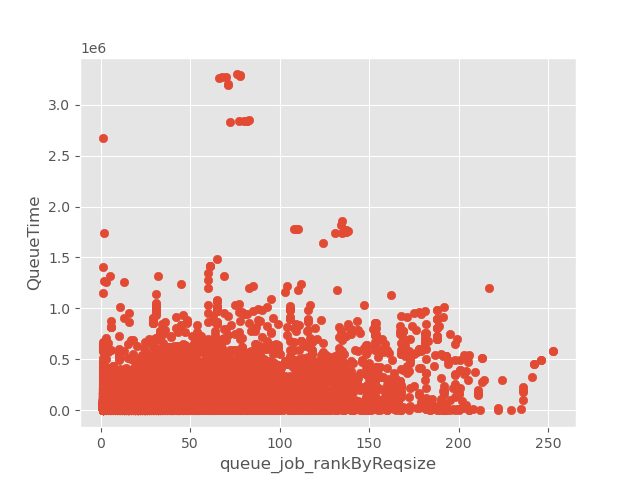
\includegraphics[width=\linewidth]{rankreqsize.png}
		\caption{scatter diagram request node rank with queue time in queue jobs list}
		\label{Fig:5}
	\end{minipage} 
\end{figure}

The results of the data analysis showed that there was not much relationship between them. Even prpjobRankReqsize is very different from what we expected. I think the reason for this is that there are a large number of small jobs use backfill queue in the theta, while most of the tasks in the default queue are large jobs and backfill has little influence. The features defined above are considered from the perspective of backfill. The allocation of queues like Theta is very unreasonable. Other supercomputer clusters do not have so many tasks to be executed on backfill queues. Subsequently, we will analyze other data sets.


\section{Progress}
In this section, we will discuss the current progress of our experiment. We first cluster the dataset and train a predictor for each cluster. When predicting a sample, we first judge its clustering category and predict it with the corresponding predictor. The details will be covered below. 

\subsection{Experimental Purpose}
We continue to use the linear model based on our previous experiments and add several features to it. The reason why linear model is used for the experiment is that for large-scale data, its convergence speed is fast, which is convenient for us to test features. At the same time, in our previous planning, we considered the combination of linear model and LSTM. However, LSTM results should only be input as a feature into the linear model, and our linear model should be able to predict without LSTM. So, our first experiment purpose is to train a linear model that could make good predictions.

In our previous plan, we wanted to combine the similarity with the model. In a recent study, A. Pal\cite{pal2021integrated} did something similar. He clustered the data sets and trained a predictor for each cluster. We used clustering on a linear model based on his idea. We use K-means for clustering. The role of clustering is actually to transform data from big heterogeneous pool to small homogeneous clusters. For dataset transformation, there are many similar  studies\cite{murali2016qespera}\cite{nurmi2007qbets}. So, the purpose of our second experiment is to use K-means to improve the accuracy of the linear model.

Finally, our final research goal is to deploy the model to the SUSTECH Taiyi cluster. Therefore, we performed data mining and data cleaning on the data from Taiyi. The obtained data was pre-processed and trained on the outside model. So, the purpose of our third experiment is to train Taiyi data on our model.

\subsection{Procedure}
[TODO...]

\subsection{Result}
[TODO...]

\subsection{Analysis and Conclusion}
[TODO...]

\section{Future Work}
[TODO...]






% trigger a \newpage just before the given reference
% number - used to balance the columns on the last page
% adjust value as needed - may need to be readjusted if
% the document is modified later
%\IEEEtriggeratref{8}
% The "triggered" command can be changed if desired:
%\IEEEtriggercmd{\enlargethispage{-5in}}

% references section

% can use a bibliography generated by BibTeX as a .bbl file
% BibTeX documentation can be easily obtained at:
% http://mirror.ctan.org/biblio/bibtex/contrib/doc/
% The IEEEtran BibTeX style support page is at:
% http://www.michaelshell.org/tex/ieeetran/bibtex/

\bibliographystyle{IEEEtran}
\bibliography{document}
% argument is your BibTeX string definitions and bibliography database(s)
%\bibliography{IEEEabrv,../bib/paper}
%
% <OR> manually copy in the resultant .bbl file
% set second argument of \begin to the number of references
% (used to reserve space for the reference number labels box)



% that's all folks
\end{document}


